
%(BEGIN_QUESTION)
% Copyright 2010, Tony R. Kuphaldt, released under the Creative Commons Attribution License (v 1.0)
% This means you may do almost anything with this work of mine, so long as you give me proper credit

A pressure instrument utilizes a {\it strain gauge} to sense pressure applied to a diaphragm.  Assuming a strain gauge resistance of precisely 23.71 k$\Omega$ at a certain applied pressure, calculate the magnitude of the voltage between points {\bf A} and {\bf B} at that pressure, and also determine the polarity of that voltage:

$$\includegraphics[width=15.5cm]{i03710x01.eps}$$

\vskip 10pt

$V$ = \underbar{\hskip 50pt} millivolts

\underbar{file i03710}
%(END_QUESTION)





%(BEGIN_ANSWER)

\noindent
5 points for voltage, 5 points for polarity:

\vskip 10pt

$V$ = 12.194 mV, with {\bf A} negative and {\bf B} positive

%(END_ANSWER)





%(BEGIN_NOTES)

{\bf This question is intended for exams only and not worksheets!}.

%(END_NOTES)


